% This is "sig-alternate.tex" V2.1 April 2013
% This file should be compiled with V2.5 of "sig-alternate.cls" May 2012
%
% This example file demonstrates the use of the 'sig-alternate.cls'
% V2.5 LaTeX2e document class file. It is for those submitting
% articles to ACM Conference Proceedings WHO DO NOT WISH TO
% STRICTLY ADHERE TO THE SIGS (PUBS-BOARD-ENDORSED) STYLE.
% The 'sig-alternate.cls' file will produce a similar-looking,
% albeit, 'tighter' paper resulting in, invariably, fewer pages.
%
% ----------------------------------------------------------------------------------------------------------------
% This .tex file (and associated .cls V2.5) produces:
%       1) The Permission Statement
%       2) The Conference (location) Info information
%       3) The Copyright Line with ACM data
%       4) NO page numbers
%
% as against the acm_proc_article-sp.cls file which
% DOES NOT produce 1) thru' 3) above.
%
% Using 'sig-alternate.cls' you have control, however, from within
% the source .tex file, over both the CopyrightYear
% (defaulted to 200X) and the ACM Copyright Data
% (defaulted to X-XXXXX-XX-X/XX/XX).
% e.g.
% \CopyrightYear{2007} will cause 2007 to appear in the copyright line.
% \crdata{0-12345-67-8/90/12} will cause 0-12345-67-8/90/12 to appear in the copyright line.
%
% ---------------------------------------------------------------------------------------------------------------
% This .tex source is an example which *does* use
% the .bib file (from which the .bbl file % is produced).
% REMEMBER HOWEVER: After having produced the .bbl file,
% and prior to final submission, you *NEED* to 'insert'
% your .bbl file into your source .tex file so as to provide
% ONE 'self-contained' source file.
%
% ================= IF YOU HAVE QUESTIONS =======================
% Questions regarding the SIGS styles, SIGS policies and
% procedures, Conferences etc. should be sent to
% Adrienne Griscti (griscti@acm.org)
%
% Technical questions _only_ to
% Gerald Murray (murray@hq.acm.org)
% ===============================================================
%
% For tracking purposes - this is V2.0 - May 2012

\documentclass{sig-alternate-05-2015}
\usepackage{graphicx}
\usepackage[usenames,dvipsnames]{color}
\usepackage{soul} 
\usepackage{booktabs}

\newcommand{\todo}[1]
  {{\scriptsize \textbf{\color{red} {#1}}}}


\graphicspath{ {} }


\begin{document}

% Copyright
\setcopyright{acmcopyright}
%\setcopyright{acmlicensed}
%\setcopyright{rightsretained}
%\setcopyright{usgov}
%\setcopyright{usgovmixed}
%\setcopyright{cagov}
%\setcopyright{cagovmixed}


% DOI
\doi{10.475/123_4}

% ISBN
\isbn{123-4567-24-567/08/06}

%Conference
%\conferenceinfo{PLDI '13}{June 16--19, 2013, Seattle, WA, USA}

%\acmPrice{\$0.00}

%
% --- Author Metadata here ---
\conferenceinfo{MSR}{2016 Austin, Texas USA}
%\CopyrightYear{2007} % Allows default copyright year (20XX) to be over-ridden - IF NEED BE.
%\crdata{0-12345-67-8/90/01}  % Allows default copyright data (0-89791-88-6/97/05) to be over-ridden - IF NEED BE.
% --- End of Author Metadata ---

\title{A deeper look into bug fixes: Patterns, replacements, deletions, and additions}

%
% You need the command \numberofauthors to handle the 'placement
% and alignment' of the authors beneath the title.
%
% For aesthetic reasons, we recommend 'three authors at a time'
% i.e. three 'name/affiliation blocks' be placed beneath the title.
%
% NOTE: You are NOT restricted in how many 'rows' of
% "name/affiliations" may appear. We just ask that you restrict
% the number of 'columns' to three.
%
% Because of the available 'opening page real-estate'
% we ask you to refrain from putting more than six authors
% (two rows with three columns) beneath the article title.
% More than six makes the first-page appear very cluttered indeed.
%
% Use the \alignauthor commands to handle the names
% and affiliations for an 'aesthetic maximum' of six authors.
% Add names, affiliations, addresses for
% the seventh etc. author(s) as the argument for the
% \additionalauthors command.
% These 'additional authors' will be output/set for you
% without further effort on your part as the last section in
% the body of your article BEFORE References or any Appendices.

\numberofauthors{3} %  in this sample file, there are a *total*
% of EIGHT authors. SIX appear on the 'first-page' (for formatting
% reasons) and the remaining two appear in the \additionalauthors section.
%
\author{
% You can go ahead and credit any number of authors here,
% e.g. one 'row of three' or two rows (consisting of one row of three
% and a second row of one, two or three).
%
% The command \alignauthor (no curly braces needed) should
% precede each author name, affiliation/snail-mail address and
% e-mail address. Additionally, tag each line of
% affiliation/address with \affaddr, and tag the
% e-mail address with \email.
%
% 1st. author
\alignauthor
Mauricio Soto\\
       \affaddr{School of Computer Science}\\
       \affaddr{Carnegie Mellon University}\\
       \affaddr{Pittsburgh, PA}\\
       \email{mauriciosoto@cmu.edu}
       % 3rd. author
\alignauthor Ferdian Thung\\
       \affaddr{Singapore Management University}\\
       \affaddr{Singapore}\\
       \email{ferdiant.2013@smu.edu.sg}
% 2nd. author
\alignauthor Chu-Pan Wong   \\
       \affaddr{Carnegie Mellon University}\\
       \affaddr{Pittsburgh, PA}\\
       \email{chupanw@cs.cmu.edu}       
\and  % use '\and' if you need 'another row' of author names
% 4th. author
\alignauthor
Claire Le Goues\\
       \affaddr{School of Computer Science}\\
       \affaddr{Carnegie Mellon University}\\
       \affaddr{Pittsburgh, PA}\\
       \email{clegoues@cs.cmu.edu}
% 5th. author
\alignauthor
David Lo\\
\affaddr{Singapore Management University}\\
\affaddr{Singapore}\\
\email{davidlo@smu.edu.sg}       
}
% There's nothing stopping you putting the seventh, eighth, etc.
% author on the opening page (as the 'third row') but we ask,
% for aesthetic reasons that you place these 'additional authors'
% in the \additional authors block, viz.
%\additionalauthors{Additional authors: John Smith (The Th{\o}rv{\"a}ld Group,
%email: {\texttt{jsmith@affiliation.org}}) and Julius P.~Kumquat
%(The Kumquat Consortium, email: {\texttt{jpkumquat@consortium.net}}).}
\date{February 2, 2016}
% Just remember to make sure that the TOTAL number of authors
% is the number that will appear on the first page PLUS the
% number that will appear in the \additionalauthors section.

\maketitle
\begin{abstract}

With the rise of automated program repair in the last couple of years, there are a lot of questions to remain unanswered. We performed a study on the Github dump of September 2015 in which we analyzed all the fixing revisions of this dataset, and found all the replacements, additions and deletions made to these files from real life projects in Github.

We found valuable information to guide automatic software repair, such as the most common and least common replacements made by human developers in order to build a successful patch; we also analyzed what are the most likely statements to replace others. 

This information will help automatic program repair tools to be more likely to find a patch and also to be more maintainable and user friendly, taking it one step closer to what humans developers do to repair their code.


\end{abstract}


%
% The code below should be generated by the tool at
% http://dl.acm.org/ccs.cfm
% Please copy and paste the code instead of the example below. 
%
\begin{CCSXML}
<ccs2012>
 <concept>
  <concept_id>10010520.10010553.10010562</concept_id>
  <concept_desc>Computer systems organization~Embedded systems</concept_desc>
  <concept_significance>500</concept_significance>
 </concept>
 <concept>
  <concept_id>10010520.10010575.10010755</concept_id>
  <concept_desc>Computer systems organization~Redundancy</concept_desc>
  <concept_significance>300</concept_significance>
 </concept>
 <concept>
  <concept_id>10010520.10010553.10010554</concept_id>
  <concept_desc>Computer systems organization~Robotics</concept_desc>
  <concept_significance>100</concept_significance>
 </concept>
 <concept>
  <concept_id>10003033.10003083.10003095</concept_id>
  <concept_desc>Networks~Network reliability</concept_desc>
  <concept_significance>100</concept_significance>
 </concept>
</ccs2012>  
\end{CCSXML}


%
% End generated code
%

%
%  Use this command to print the description
%
\printccsdesc

% We no longer use \terms command
%\terms{Theory}

\keywords{Automatic error repair; Maintainability; Human-like patches}

\section{Introduction}

Automatic bug repair is the branch of computer science that deals with
automated ways to repair errors in software. There have been several approaches
taken towards improving the different methodologies to repair bugs in software
automatically~\cite{kim2013,weimer2009,legoues2012,pan2009}. Roughly speaking,
there are two main categories of approaches. 

On the one hand, some approaches rely on mutation operators to modify the source
code~\cite{legoues2012,weimer2009}. However, we have limited knowledge about
what kinds of statements are usually modified. In this opportunity, we study the
degree to which these mutation operators apply in practice, taking as a subject
of study several million human-made bug fixes from Github. This way it will make
it more likely for automatic error repair approaches to succeed in finding a
patch for a particular error, and also, to provide automatic error repair
software with guidelines to make the patches more human-like and therefore more
readable and maintainable by human developers, as studied empirically
by~\cite{kim2013}.

On the other hand, some approaches~\cite{kim2013} search for specific patterns
and modify source code according to predefined templates. A well known approach
is PAR~\cite{kim2013}, which creates 10 different repair templates and applies
them to the buggy code in an effort to repair it. In this paper we have taken 8
out of the 10 PAR templates and tested how common they are in the repairs made
by programmers in the latest official data dump of Github as of September 2015
provided by~\cite{dyer2013}.  Our results provide evidence of how common those
patterns are in practice. We take as reference the study performed by Dongsun
Kim et al.~\cite{kim2013} in which they look for the most common ways in which
programmers patch bugs in software. The researchers developed a variation of the
tool Genprog~\cite{weimer2009,legoues2012} with several different templates
resembling patterns programmers use to patch bugs, and then performed an
empirical study to evaluate which patches do human programmers prefer.

Although automatic program repair has been well studied in the programming language
C, not much study has been done on Java. Since the programming practice between
C and Java is not trivial, we will also show some characteristics of how human
developers fix bugs in Java.

A good complement for this paper is~\cite{zhong2015}, where they look for
additions and deletions in a smaller data set. In this paper, we focus more on
the replacements, which have been left out of the analysis of~\cite{zhong2015},
and expand their results of the deletions and additions in a broader
dataset~\cite{dyer2013}.

\section{Methodology}
Our methodology is applied to the latest official data dump of Github as of
September 2015 provided by~\cite{dyer2013}. In the following subsections, we first
describe data source and objective of our study. We then describe how we detect
bug fixing patterns in PAR to find out how common they are the dataset. Last but
not least, we describe our approach to detect Delete, Replace, and Append
bug-fixing patterns.

\subsection{Data Source and Research Objective}
We used the Boa platform~\cite{dyer2013} to be able to query the Github repository
looking for patterns that humans use to patch errors in the their code. Our main
goal is to provide guidelines for automatic error fixing approaches by providing
necessary information regarding historical replace, delete and append statements
in human written patches. 

\subsection{Detecting PAR Bug Fixing Pattern}\label{sec:method}
The bug fixing patterns that we analyze in this work are adopted from Kim et
al. paper~\cite{kim2013}. The following is the description of each considered
pattern. 
\todo{Ferdian: why are we only studying 7?  It's OK to not study all of them,
  but we need to explain why.}
  \begin{enumerate}
	\item {\bf Altering method parameters (AMP)}\\
	{\bf Example:} obj.method(v1,v2) $\rightarrow$ obj.method(v1,v3)\\
	{\bf Description:} This pattern changes the input for method parameters.
	\item {\bf Calling another method with the same parameters (MSM)}\\
	{\bf Example:} obj.method1(param) $\rightarrow$ obj.method2(param)\\
	{\bf Description:} This pattern changes the method name.
	\item {\bf Calling another overloaded method with one more parameter (COM)}\\
	{\bf Example:} obj.method(v1) $\rightarrow$ obj.method(v1,v2)\\
	{\bf Description:} This pattern adds one more parameter to the method.
	\item {\bf Changing a branch condition (CBC)}\\
	{\bf Example:} if(a != b) $\rightarrow$ if(a != b \&\& c == 0)\\
	{\bf Description:} This pattern adds or removes condition.
	\item {\bf Initializing an object (IAO)}\\
	{\bf Example:} Type obj $\rightarrow$ Type obj = new Type()\\
	{\bf Description:} This pattern adds a initialization to object declaration.
	\item {\bf Adding a null checker (ANC)}\\
	{\bf Example:} obj.m1() $\rightarrow$ if(obj!=null){obj.m1()}\\
	{\bf Description:} This pattern inserts a condition to check whether an object is null or not in order to prevent unexpected state.
	\item {\bf Adding an array out of bound checker (AOB)}\\
	{\bf Example:} arr[idx]=0 $\rightarrow$ if(idx<arr.length){arr[idx]=0}\\
	{\bf Description:} This pattern inserts a condition to check that an array index is within bound right before the index is used.
	\item {\bf Adding a collection out of bound checker (COB)}\\
	{\bf Example:} x=col.get(idx) $\rightarrow$ if(idx<col.size()){x=col.get(idx)}\\
	{\bf Description:} This pattern inserts a condition to check that a collection index is within bound before it is used.
\end{enumerate}

The above patterns only cover 8 out of 10 bug fixing patterns in PAR. The other two patterns are: (1) checking that an object is an instance of a target class before casting it; and (2) replacing expression in an if condition by another expression in the same scope. Pattern (1) cannot be analyzed because Boa does not support {\em instanceof} expression. Similarly, pattern (2) requires us to track scope between pre-fix and post-fix version, which is not supported by Boa. Implementing them ourselves might be possible, but it might require too much effort than necessary. Investigating 8 out of 10 patterns should give us a good idea on how common the patterns actually are.

As mentioned before, we analyze bug fixing patterns by utilizing Boa's language
infrastructure~\cite{dyer2013}. It contains a large number of dataset and provide
a domain specific language to perform analysis on source code. Despite this
advantage, Boa still have limited capability that prevents us from performing
precise detection of bug fixing patterns. For example, it is unable to perform a
diff between two file versions, which is needed to compare the pre-fix and the
post-fix version of a buggy file. Thus, rather than finding the exact count of
bug fixing patterns, we will find an approximate count of those patterns. The
following are descriptions on how we detect each pattern.

\begin{enumerate}
\item {\bf AMP Pattern}\\
  To detect AMP pattern, for both pre-fix and post-fix version of a buggy file,
  we create a custom method call signature. This signature contains method name,
  literal parameter, and variable parameter. we consider parameter containing
  custom expression as OTHER. This is due to inexistence of function that can
  print Abstract Syntax Tree (AST) back to source code in Boa. We discard method
  signatures that appear both in pre-fix and post-fix version. We then find
  whether there exists method with the same name and the same number of
  parameters, but different parameter signatures in pre-fix and post-fix
  version. If it exists, we consider that AMP pattern is found.
	
\item {\bf MSM Pattern}\\
  To detect MSM pattern, we create method signature similar like when detecting
  AMP pattern. This time, we find whether there exists method with the exact
  same parameter signature but different name in pre-fix and post-fix
  version. If it exists, we consider that MSM pattern is found.
	
\item {\bf COM Pattern}\\
  To detect COM pattern, we create method signature similar like when detecting
  AMP and COM pattern. This time, we find whether there are exists method with
  the same name, but the number of parameters in pre-fix and post-fix version
  differs by one. If it exists, we consider that COM pattern is found.
	
\item {\bf CBC Pattern}\\
  To detect CBC pattern, we count the number of { \em logical and} and {\em
    logical or} inside if conditional expression for both pre-fix and post-fix
  version. we assume that the addition/removal of logical operators indicate
  addition/removal of condition. If there are count differences between pre-fix
  and post-fix version, we consider that CBC pattern is found.
	
\item {\bf IAO Pattern}\\
  To detect IAO pattern, we count the number of NEW expression in variable
  declaration for both pre-fix and post-fix version. If there are count
  differences between pre-fix and post-fix version, we consider that IAO pattern
  is found.
	
\item {\bf ANC Pattern}\\
  To detect ANC pattern, we count the number of if conditional expression that
  contains {\em !=null} or {\em ==null} for both pre-fix and post-fix
  version. If there are count differences between pre-fix and post-fix version,
  we consider that ANC pattern is found.
	
\item {\bf AOB Pattern}\\
  To detect AOB pattern, we count the number of if conditional expression that
  contains {\em expr<var.length} or {\em var.length>expr} for both pre-fix and
  post-fix version. If there are count differences between pre-fix and post-fix
  version, we consider that AOB pattern is found.
  
\item {\bf COB Pattern}\\
To detect COB pattern, we count the number of if conditional expression that
contains {\em expr<col.size()} or {\em col.size()>expr} for both pre-fix and
post-fix version. If there are count differences between pre-fix and post-fix
version, we consider that COB pattern is found.
	
\end{enumerate}
\todo{IMPORTANT: Ferdian, where did the results go?  Please add the results of
  the Par study into results somewhere where it fits.}


\begin{table*}
	\centering
	\resizebox{\textwidth}{100pt}{
		\begin{tabular}{|l|r|r|r|r|r|r|r|r|r|r|r|r|r|r|r|} \hline
			&Assert&Break&Continue&Do& For&If&Label&Return&Case&Switch& Synch&Throw&Try&TypeDecl&While
			\\ \hline
			
\texttt{Assert}	&-&7.48&3.76&0.53&8.30&23.05&0.31&20.04&4.90&4.62&1.30&13.50&7.23&0.03&4.95
\\ \hline
\texttt{Break} &1.00&-&4.08&0.60&9.93&26.03&0.13&25.39&2.48&1.57&1.79&8.39&11.73&0.10&6.77
\\ \hline
\texttt{Continue} &1.74&9.42&-&1.28&11.39&18.25&0.35&22.60&3.80&2.85&2.17&8.98&9.42&0.11&7.63
\\   \hline
\texttt{Do} &0.81&5.26&6.60&0.00&9.44&14.21&0.18&15.86&3.73&1.67&1.97&5.88&6.39&0.03&27.98
\\ \hline
\texttt{For} &0.86&6.28&3.19&0.79&-&22.89&0.09&21.08&5.01&3.34&1.87&10.01&10.71&0.08&13.79
\\ \hline
\texttt{If}&1.64&8.43&2.87&0.60&13.49&-&0.24&26.46&7.45&4.80&2.85&9.89&15.11&0.08&6.11
\\ \hline
\texttt{Label} &1.30&8.33&7.86&1.11&5.18&22.85&-&15.17&3.05&2.04&14.62&10.45&4.16&0.09&3.79
\\ \hline
\texttt{Return} &1.13&9.41&3.11&0.49&13.33&27.24&0.24&-&5.59&3.65&2.55&14.91&12.61&0.12&5.61
\\ \hline
\texttt{Case} &0.78&2.84&2.84&0.39&10.27&31.79&0.16&22.40&-&0.46&2.07&7.37&11.69&0.08&6.87
\\ \hline
\texttt{Switch}&1.14&2.72&3.80&0.55&11.07&34.14&0.13&21.86&0.75&-&1.53&8.65&9.02&0.05&4.58
\\ \hline
\texttt{Synch} &0.80&6.57&2.28&0.43&10.21&24.18&0.05&19.77&6.35&2.07&-&9.16&12.16&0.04&5.93
\\ \hline
\texttt{Throw} &2.11&6.57&2.58&0.48&11.87&18.84&0.17&32.28&4.64&3.30&2.74&-&10.08&0.07&4.27
\\ \hline
\texttt{Try}&0.71&7.41&3.02&0.66&11.73&27.75&0.11&23.24&5.63&2.65&2.58&8.99&-&0.09&5.42
\\ \hline
\texttt{TypeDecl} &0.00&4.51&7.52&1.00&10.28&21.05&0.50&17.79&6.02&1.75&2.01&9.27&11.53&-&6.77
\\ \hline
\texttt{While}& 0.72&8.02&3.82&1.96&23.16&19.78&0.12&16.48&6.56&3.09&1.64&6.81&7.80&0.04&-
			\\ \hline
		\end{tabular}
		}
		\caption{Likelyness to replace the statement in the first column for the statement in the top row, in Java}
\end{table*}


\subsection{Replace Query}
The replace query we designed, is a query in which we create a visitor to traverse all the fixing revisions in this repository~\cite{dyer2013}. Therefore we are analyzing only files
that were already committed and are now being reviewed to fix an error. 

We visit each statement in the previous state of that changed
file, before the change was applied and we count the amount of appearances of
the first statement we are analyzing (the one that was deleted), and then we
count the amount of appearances of the second statement we are analyzing (the
one that was inserted). We save these values, and do the same for the latest
version of the file and save these values as well.

We then compare these results to see if either the first and second statements
being analyzed increased or decreased. Depending on these we have two
conditionals:

If the amount of occurrences of the first statement decreased and the amount of
occurrences of the second statement increased on the same file, then we say that
the first statement was replaced by the second statement in that file. Likewise,
if the amount of occurrences of the first statement increased and the amount of
occurrences of the second statement decreased on the same file, we say that the
second statement was replaced by the first statement in that file. We count the
amount of files in which this happens for each of these two cases.

The numbers in the slots of Table 1, represent the percentage rate at which the elements of the leftmost column were replaced by the elements of the top row. In the first column we have the list of statements that are being replaced (faulty statements that were removed), and on the top row we have the list of statements for which that statement was replaced for (the new statement put instead). For example, if we take the intersection of row 5 (DoStatement row) and column 2 (AsserStatement column) of the data, we have a 0.81, which means that if we take all the instances in which a Do statement was replaced by something else, the amount of times that it was replaced by an Assert statement, represent a 0.81% of the times.

It is important to notice  that this analysis doesn't consider replacing an statement kind for a different version of the same statement kind, since it is counting the amount of appearances of each statement kind. So, if for example, the developer modifies the condition inside of an if statement, the amount of if statements in the file will remain the same.

\section{Results}

% (This is the old version)
% This section investigates how do developer fix bugs from three different
% perspectives. To begin with, we show some characteristics of real-world bug
% fixes.  Afterwards, we look deeper to find out what kinds of statements are
% usually added, modified or deleted by human developers to fix bugs. Lastly, we
% show how common PAR's fixing templates are in our dataset. 

This section shows our analysis results. To begin with, we discuss the dataset
we are using, and some characteristics of real-world bug fixes. Afterwards, we
provide insights for two main categories of automatic program repair approaches.
On the one hand, some approaches rely on mutation operators to
modify the source code~\cite{legoues2012,weimer2009}, but we have limited knowledge about what kinds of
statements are usually modified. Our analysis results will fill in this
knowledge gap. On the other hand, some automatic program repair approaches~\cite{kim2013} search for specific patterns and modify source code according to
predefined templates. Our results provide evidence of how common those
patterns are in practice.

\subsection{Dataset and Characteristics}

We did our analysis on the \emph{2015 September/Github} dataset on Boa. This
dataset includes $7,830,023$ Java projects with $23,229,406$ revisions. Among
all the revisions, $4,590,679$ revisions are identified by Boa as bug fixing
revisions. We hope that this population is big enough to reflect the bug fixing
practice.

The rest of this subsection shows some characteristics of real-world bug fixes.
To begin with, we are interested in:

\begin{quote}
	How many files are changed to fix a bug?
\end{quote}

To answer this question, we identify all the bug fixing revisions in our dataset
and count the number of changed files. A file was changed if (1) it was a new
file; (2) or it was modified; (3) or it was deleted. In total, $52,052,571$
files got changed. Thus, on average each bug fixing revision changes 11.3 files.
This number is surprisingly high because most automatic program repair
techniques assume that bugs are local in most cases. There could be several
reasons behind this number. It could be the case that other software artifacts
(e.g.  documentation) are updated after bug fixing. It could also be the case
that bug fixing commit also contains changes that are not related to fixing bug
(e.g. refactoring, adding new features by creating new files). To better
understand why so many files are changed, we continue to ask:

\begin{quote}
	What are the file types of those changed files?
\end{quote}

In Boa, each changed file is represented by a \emph{ChangedFile} node, and it
has a field called \emph{FileKind}, describing the type of each file. As
mentioned earlier, a \emph{ChangedFile} could be either a new file or an
existing file (if the bug fixing revision modified or deleted the file).
Table~\ref{tbl:fileType} shows the file types that Boa could identify. To answer
this question, we iterate all the changed files in each bug fixing revision and
count the total number for each file type. Results are shown in
Table~\ref{tbl:fileType}.

\begin{table}
\centering
  \begin{tabular}{| c | r | r |}
  \hline
  File Kind & Total Number & Average \\ \hline \hline
  BINARY & 752,945 & 0.16 \\ \hline
  SOURCE\_JAVA\_ERROR & 2,073,558 & 0.45 \\ \hline
  SOURCE\_JAVA\_JLS2 & 2,607,413 & 0.57 \\ \hline
  SOURCE\_JAVA\_JLS3 & 15,748,967 & 3.43 \\ \hline
  SOURCE\_JAVA\_JLS4 & 83,798 & 0.02 \\ \hline
  TEXT & 541,023 & 0.12 \\ \hline
  XML & 6,818,299 & 1.49 \\ \hline
  UNKNOWN & 23,426,568 & 5.10 \\ \hline
  \end{tabular}
  \caption{File Types of Changed Files}
  \label{tbl:fileType}
\end{table}

\emph{SOURCE\_JAVA\_ERROR} file kind represents files that Boa failed to parse.
\emph{JLS2} refers to Java files that are written in all versions of Java
languages up to and including J2SE 1.4. \emph{JLS3} refers to J2SE 1.5, and JLS4
refers to J2SE 1.6 and 1.7. Boa documentation does not explicitly explain what
is \emph{TEXT} and what is \emph{UNKNOWN}. Our assumption is that \emph{TEXT}
refers to files whose file name ends with ``.txt'', and \emph{UNKNOWN} refers to
all other kinds of files (e.g. .c file, .cpp files).

From Table~\ref{tbl:fileType}, we can see that \emph{TEXT} files and
\emph{BINARY} files are changed least frequently. This is not surprising because
\emph{TEXT} files are usually documentation files, and \emph{BINARY} files
should only be changed in rare case (e.g.  milestone, new release, dependency
update). If we consider all 4 kinds of Java files as one kind, then on average
each bug fixing revision changes $4.47$ Java files. But still, it does not
conform to our assumption of bug locality. \emph{XML} files in Java projects
usually represents build files, thus changing one build file after each bug
fixing is not surprising.  What surprises us is that \emph{UNKNOWN} files are
changed most frequently. Note that all the projects in our dataset are Java
projects, so it is reasonable to assume that these files are not source files
that written in other programming languages.  One possible explanation is that
they are test resources. However, due to the limitations of Boa, we can not look
into the content of these \emph{UNKNOWN} files. 

Since Boa does not distinguish Java files that related to functionality and Java
files that related to testing, it could be the case that among those $4.47$
changed Java files, some of them are related to testing, such as modifying the
test cases and creating new test classes. To better understand what changes are
usually made to Java source code files, we continue to ask:

\begin{quote}
	How often do developers introduce new classes, methods, fields, variables in
	bug fixing commits?
\end{quote}

This research question is interesting because most automatic program repair
approaches often do not create new classes/methods/fields/variables to fix bugs.
Most approaches guess and synthesize the patches based on existing source code.

Table~\ref{tbl:new} shows our analysis results. This table shows that
introducing new classes and new variables are rare. This is good news for
automatic program repair approaches. On average, we still have $0.69$ new method
per bug fix. If we consider the possibility of creating new test method (i.e.
methods that annotated by @Test if JUnit is used), this number is not that
scary. However, what surprises us is that $1.32$ fields are created per bug fix.
This indicates that automatic program repair approaches should pay attention to
the state of the class when fixing Java programs.

\begin{table}
\centering
  \begin{tabular}{| c | r | r |}
  \hline
  Introducing & Total Number & Average \\ \hline \hline
  Class & 729,201 & 0.16 \\ \hline
  Methods & 3,186,867 & 0.69 \\ \hline
  Fields & 6,076,646 & 1.32 \\ \hline
  Variables & 924,259 & 0.2 \\ \hline
  \end{tabular}
  \caption{Introducing new classes, methods, fields, variables to fix bugs}
  \label{tbl:new}
\end{table}

% \todo{Is there room/call to include any element of Chu Pan's replacement
%   analysis in here?}


\subsection{What changes are common in real-world bug fixes?}

Most automatic program repair approaches mutate source code using predefined
mutation operators, which represent different ways of modifying source code. In
order to generate patches that make more sense to human developers, it would be
beneficial to first investigate how developers mutate source code to fix bugs. 

For each bug fixing revision $r$ and each statement kind $k$, we count how many
statements of kind $k$ are there in revision $r$ and $r-1$ ($r-1$ means the
revision before revision $r$), and then compare the two numbers. For example, if
the number of if statements in revision $r$ is more than the number in revision
$r-1$, we say bug fixing revision $r$ introduce new if statements. Note that
``introducing new if statements'' does not necessarily mean human developers
introduce them to fix bugs. However, our hope is that this analysis could still
provide us some hints, given the large number of bug fixing revisions we are
analyzing.

\begin{figure*}[!t] \centering
	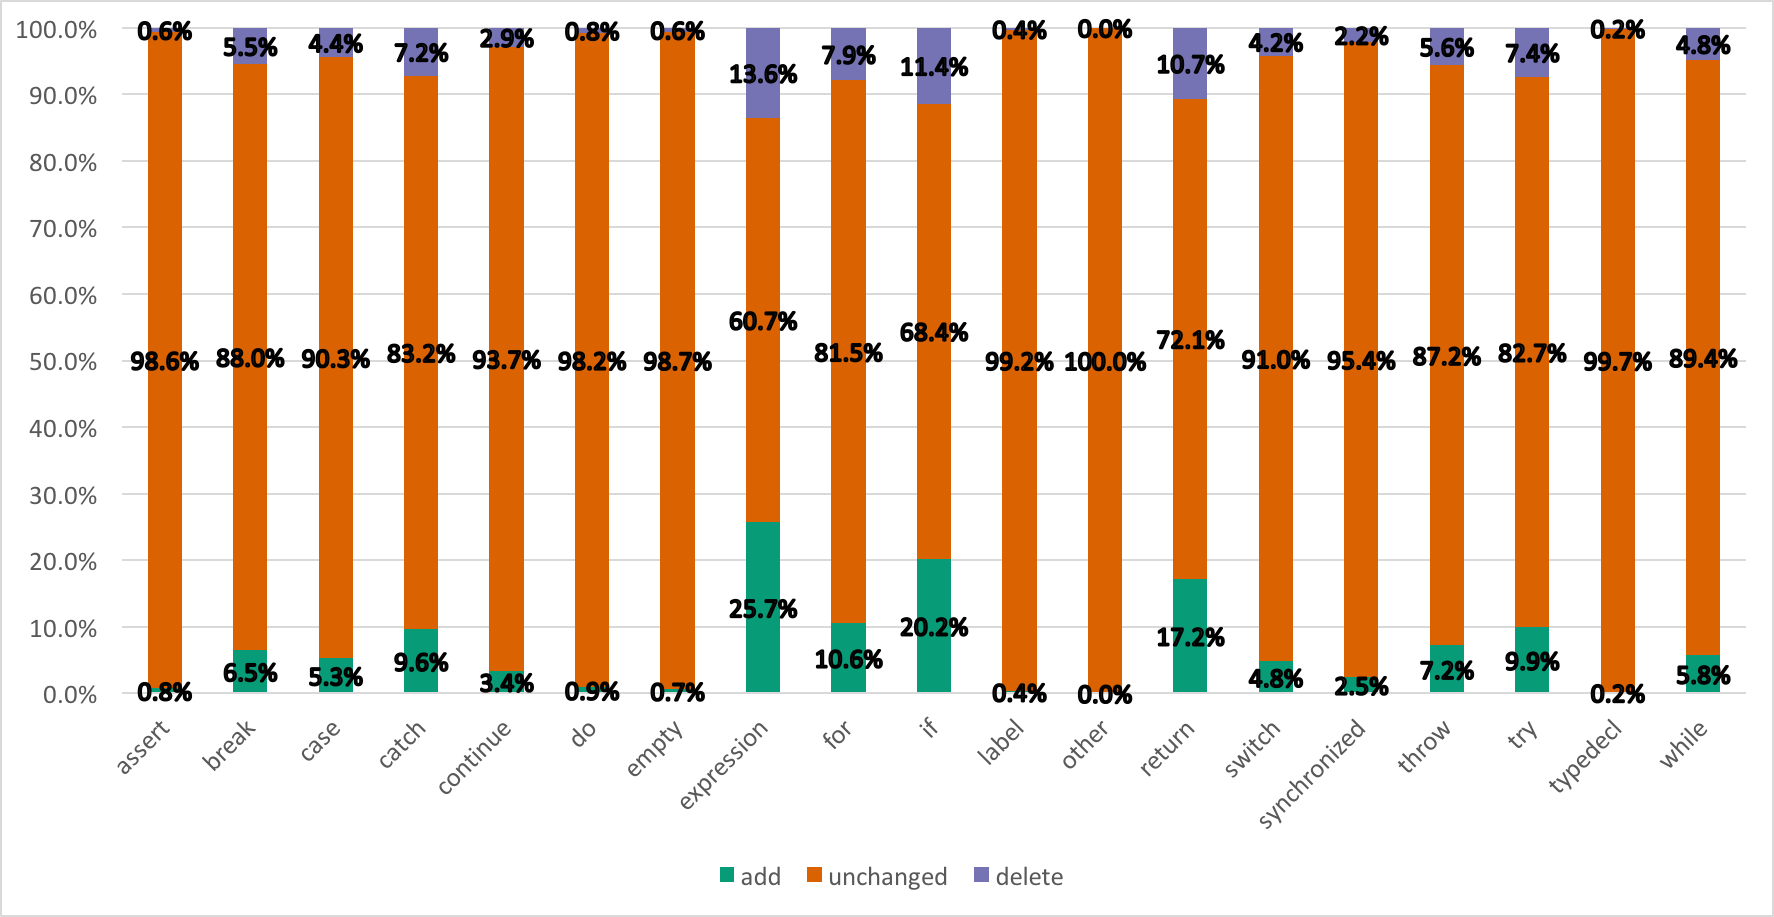
\includegraphics[width=0.95\textwidth]{StmtType} \caption{For each kind
	of statement, how many bug fixing revisions add/delete statements of the
same kind?} \label{fig:StmtType} \end{figure*}

From Figure~\ref{fig:StmtType} \todo{fix the small fonts in this graph}, we can
see that expression, if, return, for and try catch statements are added most
often. On the other hand, the same types of statements are also deleted most
often. This finding indicates that most bugs were fixed by changing the control
flow of the program using if, return, for, while, and try catch statements. 

For each bug fixing revision, the results discussed above consider both newly
added files and existing files. Since most automatic program repair approaches
do not generate new files to fix bugs, the rest of this section only considers
files that were already in the repositories when developers fixed bugs. Our
analysis shows that there are 46,301,429 of them. In these files, there is a
total of 517,281 statement kinds being replaced, and 511,198 replacing these
statements kinds.

We analyzed each of these files looking for statement kinds being either replaced by other kinds, deleted or appended to the file.

We found that the most common Replacer statement kind, meaning the statement
kind that most commonly replaces others is the \textbf{If Statement} with
101,366 appearances. The least common Replacer, meaning the statement kind which
is less likely to replace other statement kinds is the \textbf{Type Declaration
  Statement} with 447 appearances.

The most common Replacee, which is the most likely statement kind to be replaced
by another statement kind is the \textbf{Return Statement} with 111,938
appearances. The least common Replacee, which is the least common statement to
be replaced by another statement kind is the \textbf{Type Declaration Statement}
with 399 appearances.

\subsubsection{Likeliness of replacement}
This study is directly applicable to automatic software repair. Most common
tools for automatic software repair~\cite{kim2013,weimer2009,legoues2012}
first find a faulty statement using several different fault localization
techniques~\cite{fry2010}, and once they have that faulty statement, they apply
different kinds of edits to it, usually at random. Which makes it equally likely
to replace an statement for another without looking at the kinds of statements
being replaced.

With this study, we are able to make a more accurate guess, when having a known faulty statement, to which statement it is more likely to replace it for. By taking a look at the data of Table 1, we can find the most likely replacements that will end up being a successful patch. 

For example, if we are fixing a Java program, and we have a faulty statement that happens to be a For Statement. Then we can look up in Table 1 the For Statement Row (6th row), and take a look at the probability of that statement to be replaced by other kinds of statement. In this example we see that the top 3 most likely statements to replace a For Statement are an If statement with a 22.89\% likeliness, followed by a return statement with a 21.08\%, and third is a While statement with a 13.79\% of likeliness to replace a For Statement. This way we know that it is more likely for a programmer to replace a For Statement for those three different kinds of statements and this provides guidelines to the automatic bug repair approaches to consider this on their effort to find a patch.

\subsubsection{Most common replacements}
Our results show that the most common replacement is when developers remove a Return statement and insert an If statement. This showed up in 30,489 files in the code database. The second most common replacement is removing an If statement and insert a Return statement instead, which had 28,536 appearances in the code database. Third to that, is to remove a Return statement and insert a Throw statement.

\subsubsection{Least common replacements}
On the opposite side of the data, we can see that the least common replacement was an Assert statement replacing a Type Declaration statement. This was the only replacement to have zero appearances in our search through the 46,301,429 files being fixed. Close to it, as the second least common replacement was removing a Do statement and insert a Type Declaration statement, with one appearance in our code database, and on third place, removing a Label and insert a Type Declaration Statement had one appearance in our code database.

\subsection{How common are the fixing templates of PAR?}\label{sec:freqfixpattern}
After running the bug pattern detection approach on Boa's dataset, I obtained the result shown in Table~\ref{tab:freqpattern}. The result shows that AMC, MSM, COM, CBC, IAO, ANC, AOB, and COB pattern is found on 1.95\%, 1.69\%, 0.58\%, 4.23\%, 2.82\%, 2.90\%, 0.28\%, and 0.57\% of buggy files. We can see that the most common pattern among these patterns is CBC and the least common pattern is AOB. If we assume that these patterns never appear together in the dataset, these patterns cover 14.78\% of buggy files. Kim et al. mentioned that the patterns that they use cover almost 30\% of real patches~\cite{kim2013}. Although we only detect 8 out of 10 bug fixing patterns, it is hard to believe that the remaining two patterns cover 15\% of buggy files, especially 14.78\% is a number we get when we assume that the patterns that we detect never appear together. Moreover, the percentage of each pattern is based on imprecise approximation which is likely to represent an upper bound rather than a lower bound. This suggests that common bug fixing patterns might not be as common as it appeared to be.

\begin{table}[!htb]
	\caption{Frequency of Bug Fixing Patterns}\label{tab:freqpattern}
	\centering
	\begin{tabular}{lr} 
		\hline
		& \textbf{GitHub}\\
		\hline
		\#Buggy Files & 46,301,429 \\ 
		\#AMP Pattern & 901,083 \\
		\#MSM Pattern & 783,073 \\
		\#COM Pattern & 270,128 \\ 
		\#CBC Pattern & 1,959,377 \\  
		\#IAO Pattern & 1,308,006 \\  
		\#ANC Pattern & 1,340,561 \\  
		\#AOB Pattern & 128,016 \\  
		\#COB Pattern & 262,915 \\   
		\hline
	\end{tabular}
\end{table}

\section{Threats to Validity} 

Since we are using a DSL provided by Boa to implement our analysis, the
correctness of our analysis depends on our programs as well as Boa itself. To
prevent errors from our side, we open source our implementation on
Github~\footnote{\url{https://github.com/}}.\todo{update
this}

Some threats to our study are due to the limitation of Boa. For example, we rely
on Boa to identify bug fixing revisions, but it is unclear whether those
identified revisions are actually related to bug fixing. Chances are that there
exist some other bug fixing revisions, but Boa could not identify them. It is
also possible that bug fixing revisions identified by Boa actually include other
code changes, such as implementing new features, refactoring the code base.
After all, identifying bug fixing revisions from revision history is still an
open problem. Another big limitation of Boa is that there is no easy to get a
precise statement-level diff between two revisions. Thus, our template matching
and analysis of code changes (by counting each statement kind) could be
inaccurate. However, our results should provide upper bounds for the questions
we investigated. 

\section{Conclusions}
The findings of our study provide a set of useful guidelines for automatic
program repair tools with which their search for a patch can be now improved by
having the knowledge of how likely it is to replace a faulty statement by the
different kinds of statements available.
\todo{Expand to include summary of actual conclusions}


%\end{document}  % This is where a 'short' article might terminate



\bibliographystyle{abbrv}
\bibliography{sigproc}  % sigproc.bib is the name of the Bibliography in this case
% You must have a proper ".bib" file
%  and remember to run:
% latex bibtex latex latex
% to resolve all references
%
% ACM needs 'a single self-contained file'!
%
%APPENDICES are optional
%\balancecolumns


%\balancecolumns % GM June 2007
% That's all folks!
\end{document}
